
This analysis uses several different control regions in addition to the signal regions. 
All of these different regions are defined in this section. 
%Figure~\ref{fig:venndiagram} illustrates the relationship between these regions.

\subsection{Single Lepton Selection}

[UPDATE SELECTION]

The single lepton preselection sample is based on the following criteria
\begin{itemize}
\item satisfy the trigger requirement (see
  Table.~\ref{tab:DatasetsData}). Dilepton triggers are used only for the dilepton control region.
\item select events with one high \pt\ electron or muon, requiring
  \begin{itemize}
  \item $\pt>30~\GeVc$ and $|\eta|<2.1$
  \item satisfy the identification and isolation requirements detailed
    in the same-sign SUSY analysis (SUS-11-010) for electrons and the opposite-sign 
    SUSY analysis (SUS-11-011) for muons
  \end{itemize} 
  \item require at least 4 PF jets in the event with $\pt>30~\GeV$
    within $|\eta|<2.5$ out of which at least 1 satisfies the CSV
    medium working point b-tagging requirement
  \item require moderate $\met>50~\GeV$
\end{itemize}

Table~\ref{tab:preselectionyield} shows the yields in data and MC without any corrections for this preselection region.

\begin{table}[!h]
\begin{center}
\begin{tabular}{c|c}
\hline
\hline
\end{tabular}
\caption{  Raw Data and MC predictions without any corrections are shown after preselection. \label{tab:preselectionyield}}
\end{center}
\end{table}

\subsection{Signal Region Selection}

[MOTIVATIONAL BLURB ON MET AND MT, \\
CAN ADD SIGNAL VS. TTBAR MC PLOT \\
ADD SIGNAL YIELDS FOR AVAILABLE POINTS, \\
DISCUSS CHOICE SIG REGIONS]

The signal regions (SRs) are selected to improve the sensitivity for the
single lepton requirements and cover a range of scalar top
scenarios. The \mt\ and \met\ variables are used to define the signal
regions and the requirements are listed in Table~\ref{tab:srdef}. 

\begin{table}[!h]
\begin{center}
\begin{tabular}{l|c|c}
\hline
Signal Region & Minimum \mt\ [GeV] & Minimum \met\ [GeV] \\
\hline
\hline
SRA & 150 & 100 \\
SRB & 120 & 150 \\
SRC & 120 & 200 \\
SRD & 120 & 250 \\
SRE & 120 & 300 \\
\hline
\end{tabular}
\caption{ Signal region definitions based on \mt\ and \met\
  requirements. These requirements are applied in addition to the
  baseline single lepton selection.
\label{tab:srdef}}
\end{center}
\end{table}

Table~\ref{tab:srrawmcyields} shows the expected number of SM
background yields for the SRs. A few stop signal yields for four
values of the parameters are also shown for comparison. The signal
regions with looser requirements are sensitive to lower stop masses
M(\sctop), while those with tighter requirements are more sensitive to
higher M(\sctop). 

\begin{table}[!h]
\begin{center}
\begin{tabular}{l||c|c|c|c}
\hline
Sample              & SRA & SRB & SRC & SRD \\
\hline
\hline
\ttdl\ 		 & $700 \pm 15$& $408 \pm 12$& $134 \pm 7$& $43 \pm 4$ \\
\ttsl\ \& single top (1\Lep) 		 & $111 \pm 6$& $71 \pm 5$& $15 \pm 2$& $4 \pm 1$ \\
\wjets\ 		 & $58 \pm 35$& $57 \pm 35$& $29 \pm 26$& $26 \pm 26$ \\
Rare 		 & $63 \pm 3$& $40 \pm 3$& $17 \pm 2$& $7 \pm 1$ \\
\hline
Total 		 & $932 \pm 39$& $576 \pm 38$& $195 \pm 27$& $80 \pm 26$ \\
\hline
\end{tabular}
\caption{ Expected SM background contributions, including both muon
  and electron channels. The uncertainties are statistical only. ADD
  SIGNAL POINTS.
\label{tab:srrawmcyields}}
\end{center}
\end{table}

\subsection{Control Region Selection}

[1 PARAGRAPH BLURB RELATING BACKGROUNDS (IN TABLE FROM PREVIOUS SECTION)
TO INTRODUCE CONTROL REGIONS]

Control regions (CRs) are used to validate the background estimation
procedure and derive systematic uncertainties for some
contributions. The CRs are selected to have similar
kinematics to the SRs, but have a different requirement in terms of
number of b-tags and number of leptons, thus enhancing them in
different SM contributions. The four CRs used in this analysis are
summarized in Table~\ref{tab:crdef}.

\begin{table}
\begin{center}
{\small
\begin{tabular}{l|c|c|c}
\hline
Selection 	& \multirow{2}{*}{exactly 1 lepton}	& \multirow{2}{*}{exactly 2
	leptons}		& \multirow{2}{*}{1 lepton + isolated
        track}\\
      Criteria & & & \\
\hline
\hline
\multirow{4}{*}{0 b-tags} 	 
& 	 CR1) W+Jets dominated:
& 	 CR2) apply \Z-mass constraint			 
& 	 CR3) not used \\  
& 	 
&       $\rightarrow$ Z+Jets dominated: Validate 
&      \\
&      Validate W+Jets \mt\ tail
& 	 \ttsl\ \mt\ tail comparing 
& 	 \\  
&
& 	 data vs. MC ``pseudo-\mt ''
& 	 \\  
\hline
\multirow{4}{*}{$\ge$ 1 b-tags} 	 
& 	
& 	CR4) Apply \Z-mass veto 
&      CR5) \ttdl, \ttlt\ and \\
&     SIGNAL 
&      $\rightarrow$ \ttdl\ dominated: Validate 
&	\ttlf\ dominated:  Validate \\
&     REGION 
&      ``physics'' modelling of \ttdl\     
&      \Tau\  and fake lepton modeling/\\
&
&
&      detector effects in \ttdl\     \\
\hline
\end{tabular}
}
\caption{Summary of signal and control regions.
  \label{tab:crdef}%\protect
}
\end{center}
\end{table}


\subsection{MC Corrections}

[UPDATE SECTION]

\subsubsection{Corrections to Jets and \met}

[UPDATE, ADD FEW MORE DETAILS ON WHAT IS DONE HERE]

The official recommendations from the Jet/MET group are used for 
the data and MC samples. In particular, the jet
energy corrections (JEC) are updated using the official recipe.
L1FastL2L3Residual (L1FastL2L3) corrections are applied for data (MC),
based on the global tags GR\_R\_42\_V23 (DESIGN42\_V17) for
data (MC). In addition, these jet energy corrections are propagated to
the \met\ calculation, following the official prescription for
deriving the Type I corrections. 

Events with anomalous ``rho'' pile-up corrections are excluded from the sample since these 
correspond to events with unphysically large \met\ and \mt\ tail
signal region. In addition, the recommended MET filters are applied. 


\subsubsection{Branching Fraction Correction}

The leptonic branching fraction used in some of the \ttbar\ MC samples
differs from the value listed in the PDG $(10.80 \pm 0.09)\%$. 
Table.~\ref{tab:wlepbf} summarizes the branching fractions used in
the generation of the various \ttbar\ MC samples. 
For \ttbar\ samples with the incorrect leptonic branching fraction, event
weights are applied based on the number of true leptons and the ratio
of the corrected and incorrect branching fractions. 

\begin{table}[!h]
\begin{center}
\begin{tabular}{c|c}
\hline
         \ttbar\ Sample - Event Generator & Leptonic Branching Fraction\\
\hline
\hline
Madgraph   &       0.111\\
MC@NLO    &       0.111\\
Pythia         &       0.108\\
Powheg       &       0.108\\
\hline
\end{tabular}
\caption{Leptonic branching fractions for the various \ttbar\ samples
  used in the analysis. The primary \ttbar\ MC sample produced with
  Madgraph has a branching fraction that is almost $3\%$ higher than
  the PDG value. \label{tab:wlepbf}}
\end{center}
\end{table}


\subsubsection{Modeling of Additional Hard Jets in Top Dilepton Events}
\label{sec:jetmultiplicity}

[CHECK, UPDATE, ADD EQUATIONS COMMENTED IN THE BOTTOM OF FILE \\
REFERENCE APPENDIX INFO. (FROM 7 TEV) AND SUMMARIZE THAT INFORMATION HERE]

Dilepton \ttbar\ events have 2 jets from the top decays, so additional
jets from radiation or higher order contributions are required to
enter the signal sample. The modeling of addtional jets in \ttbar\
events is checked in a \ttll\ control sample,
selected by requiring
\begin{itemize}
\item exactly 2 selected electrons or muons with \pt $>$ 20 GeV
\item \met\ $>$ 100 GeV
\item $\geq1$ b-tagged jet
\item Z-veto 
\end{itemize}
Figure~\ref{fig:dileptonnjets} shows a comparison of the jet
multiplicity distribution in data and MC for this two-lepton control
sample. After requiring at least 1 b-tagged jet, most of the
events have 2 jets, as expected from the dominant process \ttll. There is also a
significant fraction of events with additional jets. 
The 3-jet sample is mainly comprised of \ttbar\ events with 1 additional
emission and similarly the $\ge4$-jet sample contains primarily
$\ttbar+\ge2$ jet events. 
%Even though the primary \ttbar\
%Madgraph sample used includes up to 3 additional partons at the Matrix
%Element level, which are intended to describe additional hard jets,
%Figure~\ref{fig:dileptonnjets} shows a slight mis-modeling of the
%additional jets. 


\begin{figure}[hbt]
  \begin{center}
	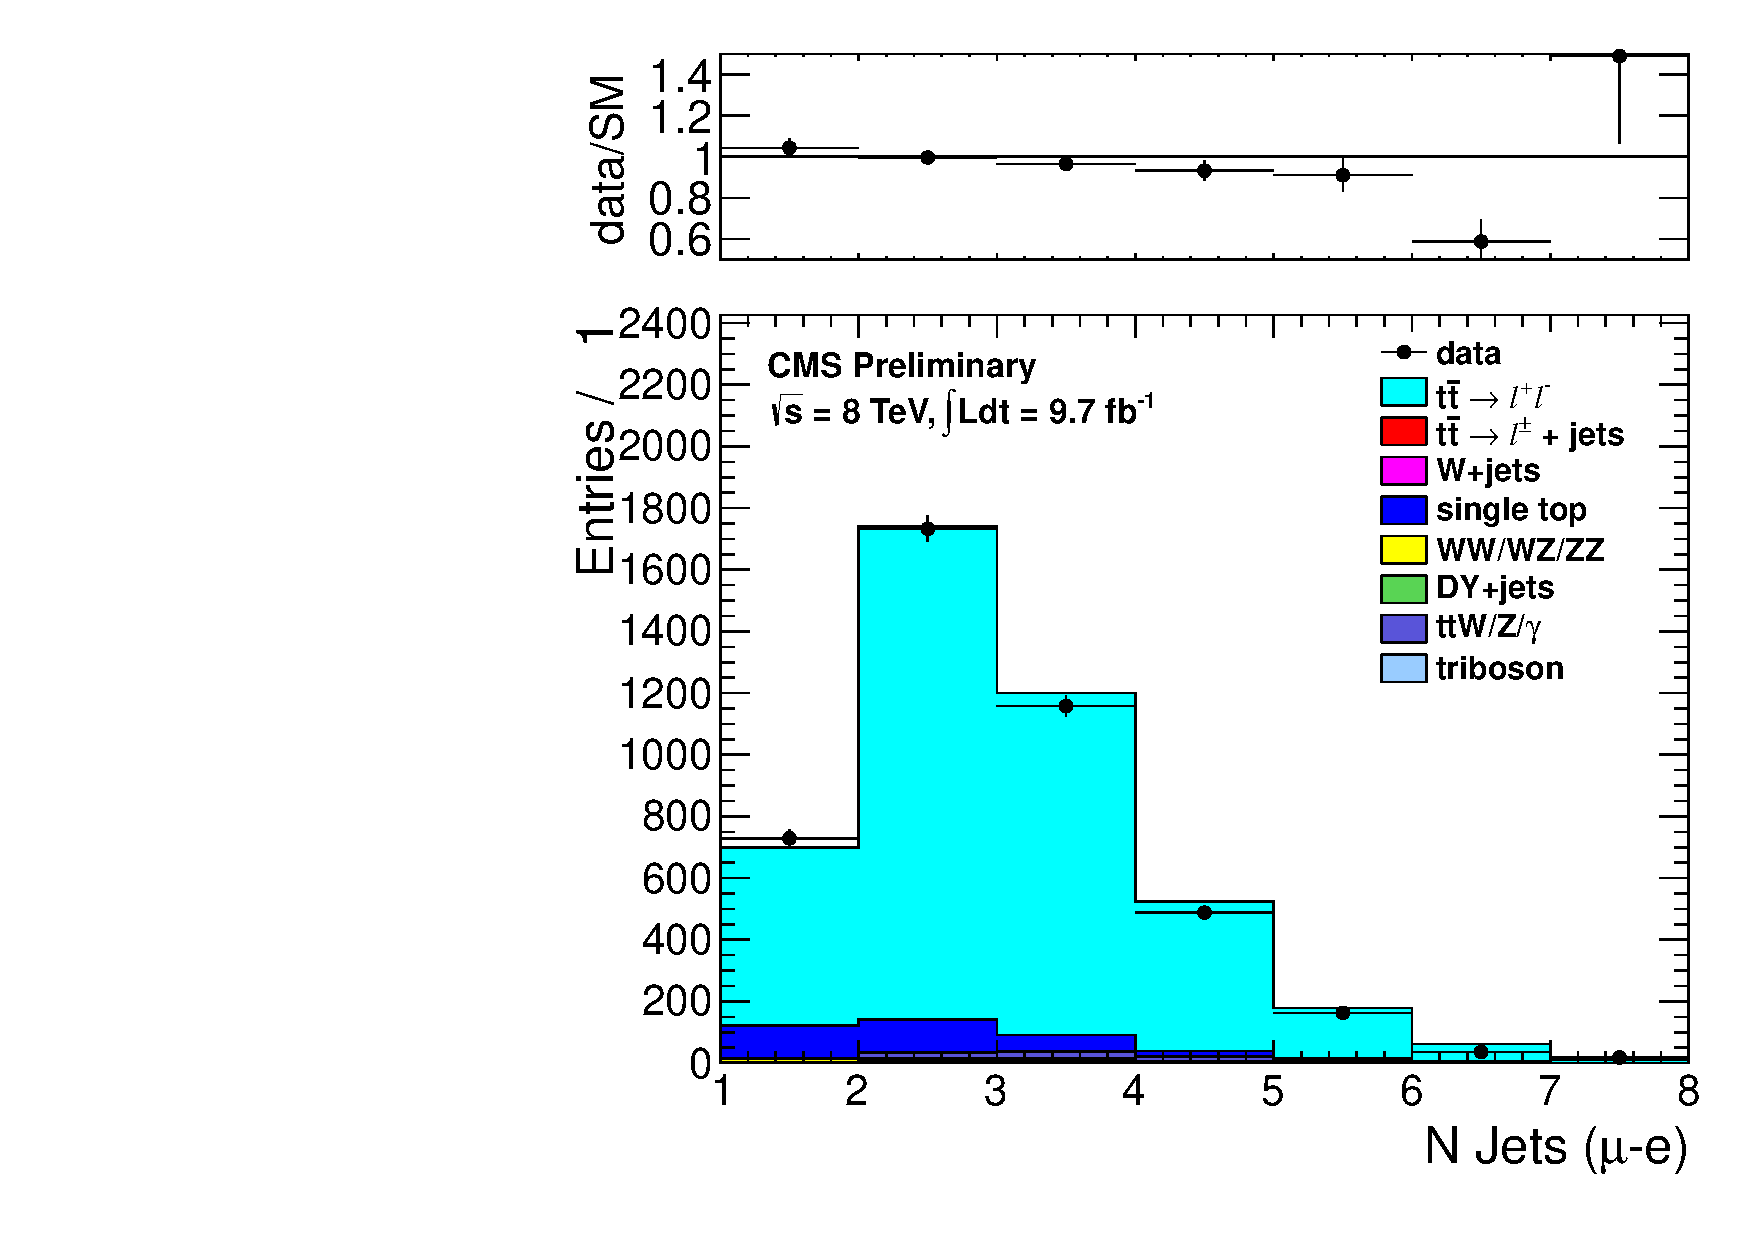
\includegraphics[width=0.5\linewidth]{plots/njets_all_met100_mueg.pdf}
	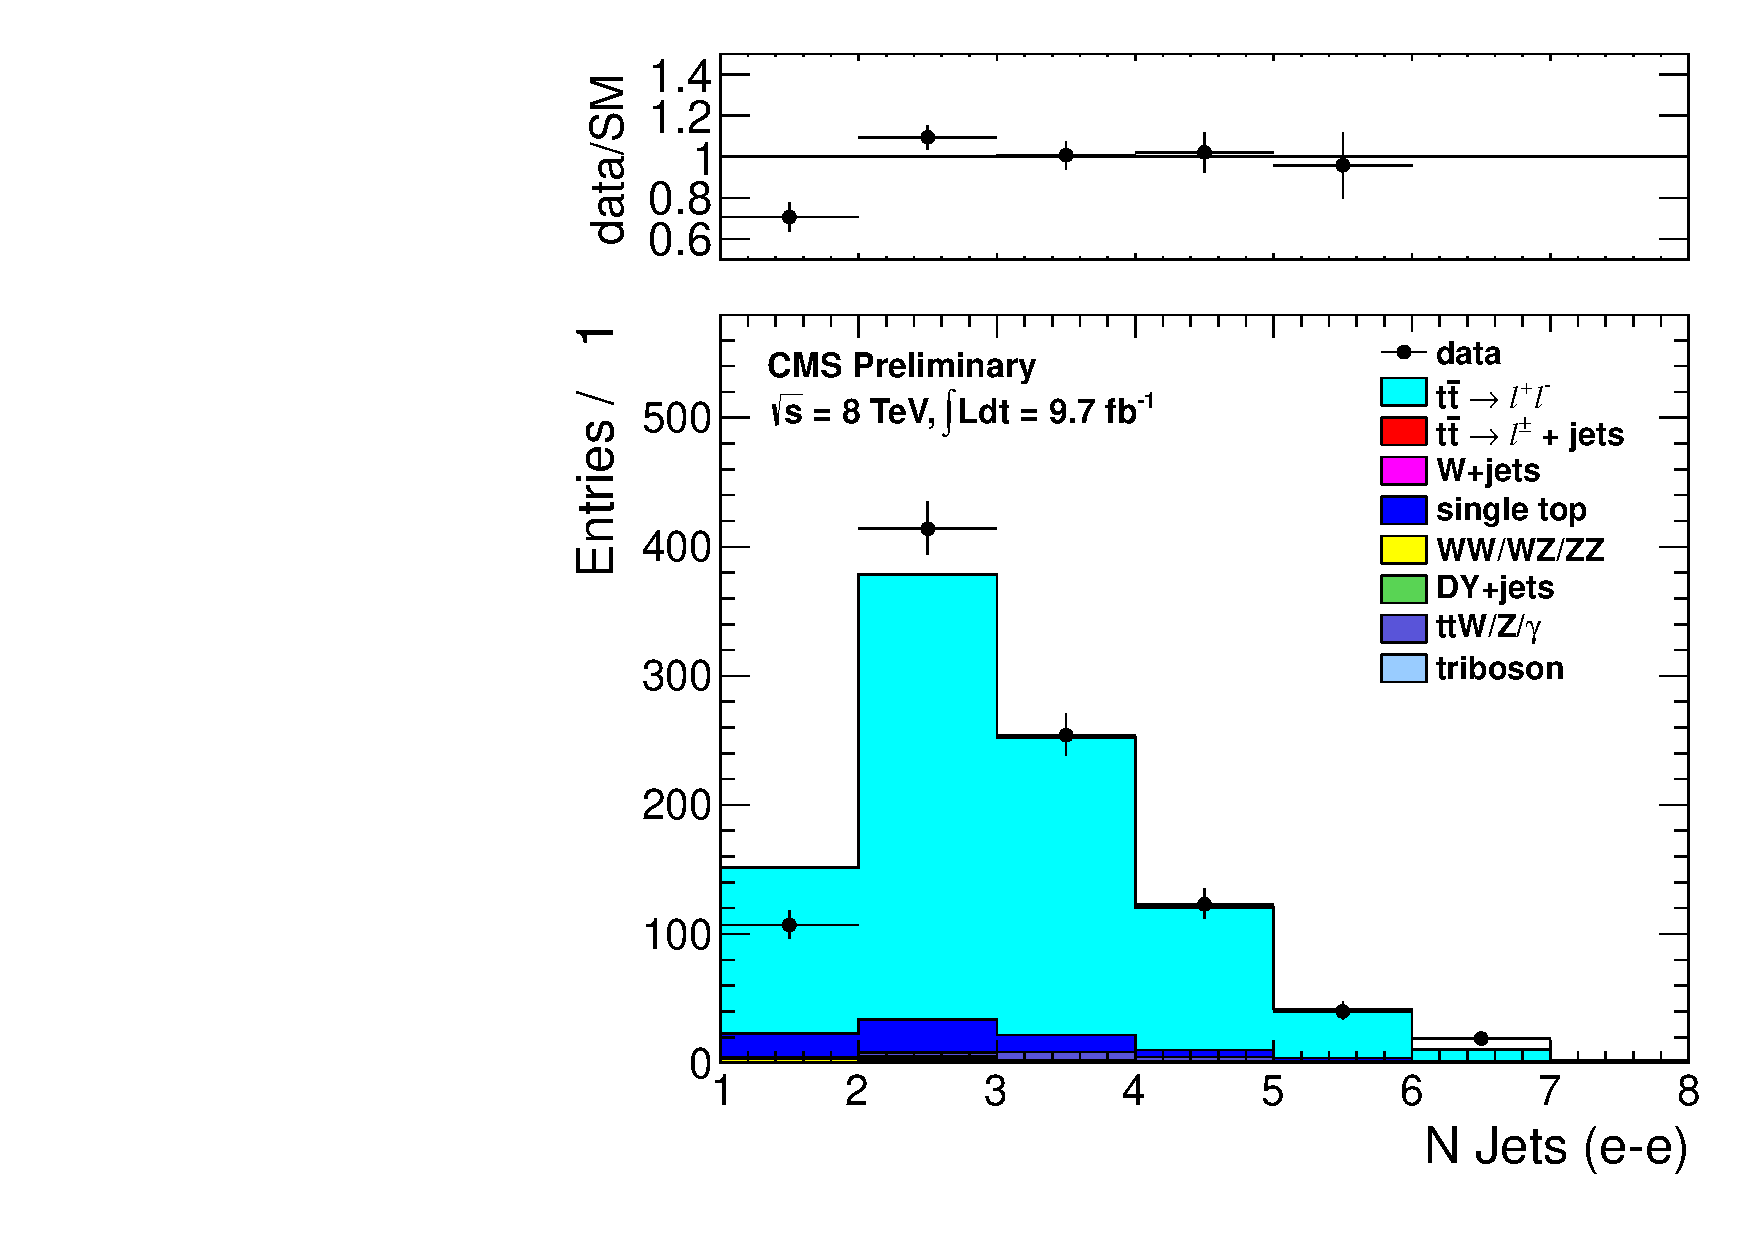
\includegraphics[width=0.5\linewidth]{plots/njets_all_met100_diel.pdf}%
        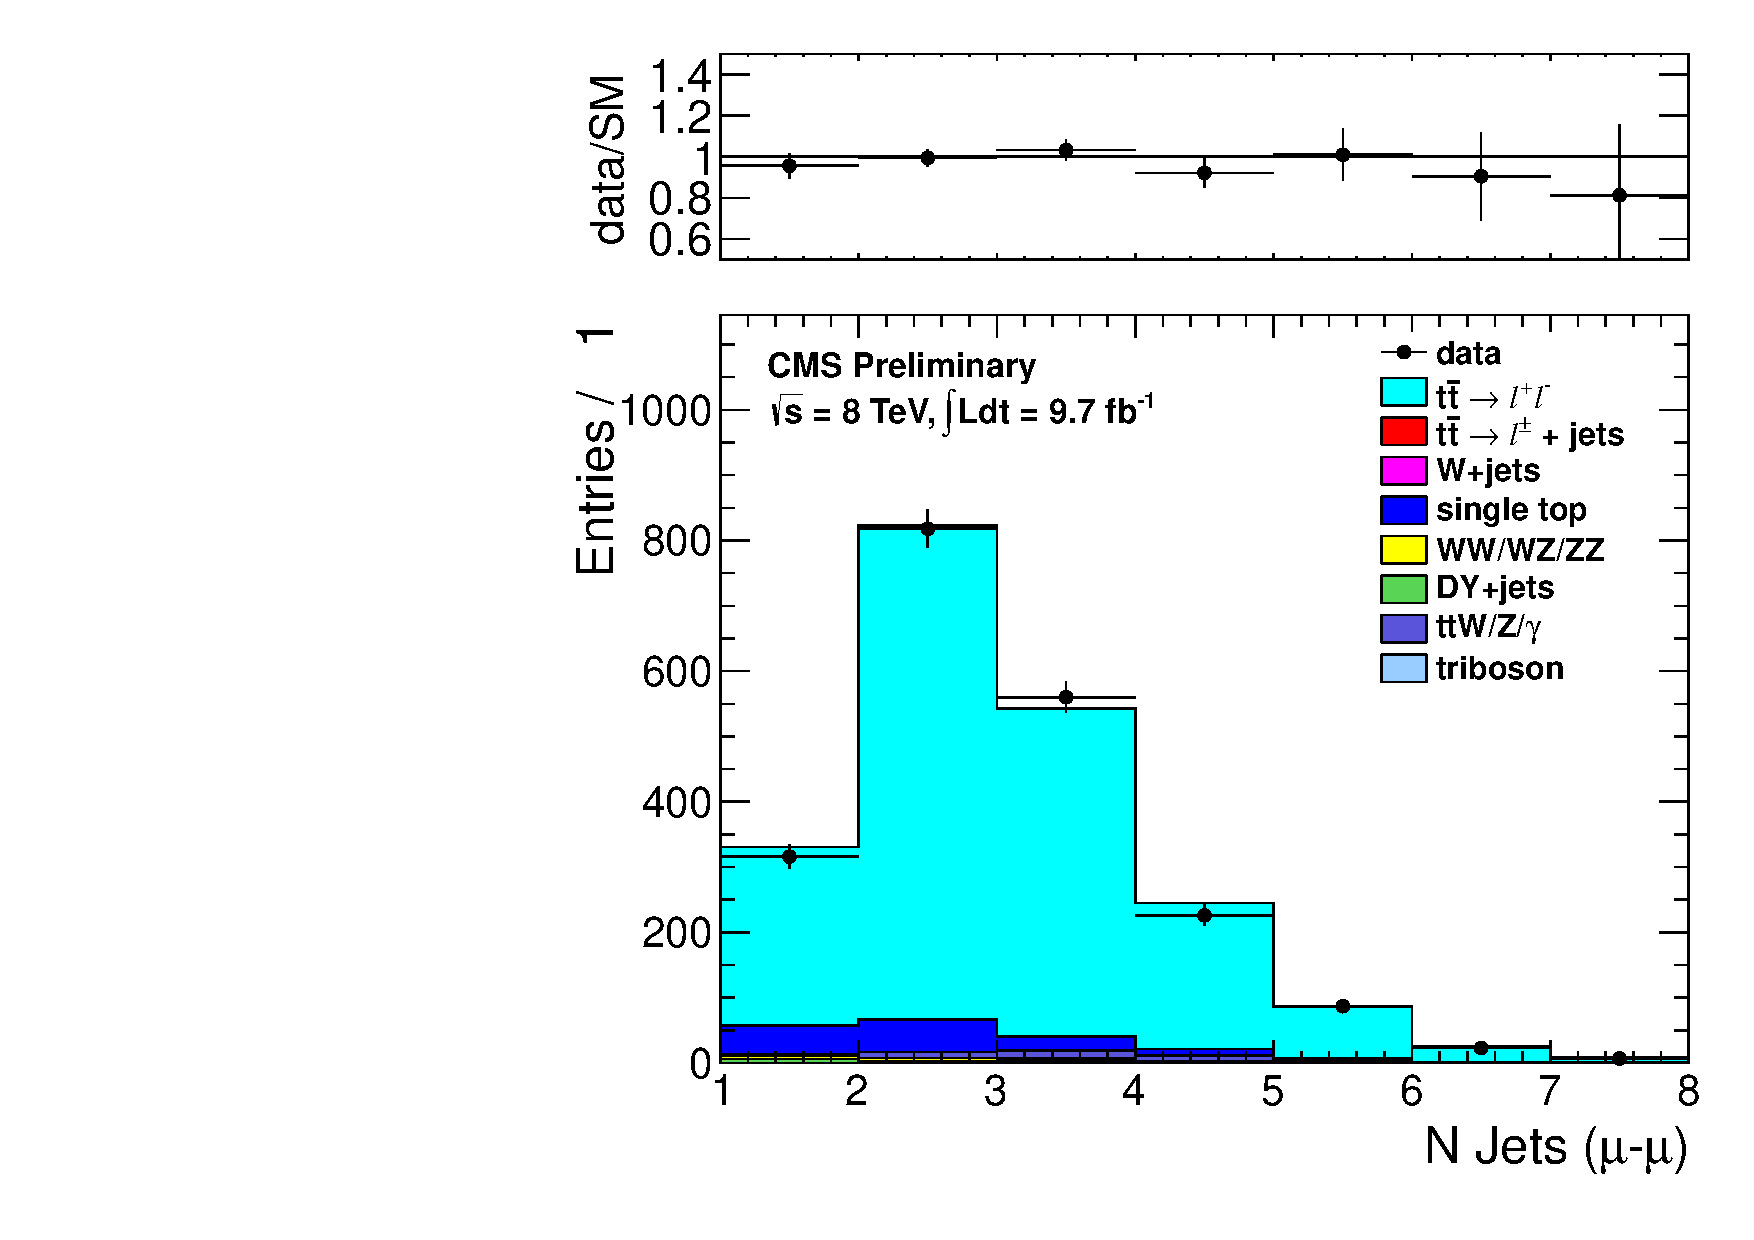
\includegraphics[width=0.5\linewidth]{plots/njets_all_met100_dimu.pdf}
	\caption{
	  \label{fig:dileptonnjets}%\protect 
          Comparison of the jet multiplicity distribution in data and MC for dilepton events in the \E-\M\
          (top), \E-\E\ (bottom left) and \M-\M\ (bottom right) channels.}  
      \end{center}
\end{figure}

It should be noted that in the case of \ttll\ events
with a single reconstructed lepton, the other lepton may be
mis-reconstructed as a jet. For example, a hadronic tau may be
mis-identified as a jet (since no $\tau$ identification is used). 
In this case only 1 additional jet from radiation may suffice for 
a \ttll\ event to enter the signal sample. As a result, both the
samples with $\ttbar+1$ jet and $\ttbar+\ge2$ jets are relevant for
estimating the top dilepton bkg in the signal region.

%In this section we discuss a correction to $ N_{2 lep}^{MC} $ in Equation XXX
%due to differences in the modelling of the jet multiplicity in data versus MC.
%The same correction also enters $ N_{peak}^{MC}$ in Equation XXX to the extend that the 
%dilepton contributions to $ N_{peak}^{MC}$ gets corrected.

%The dilepton control sample is defined by the following requirements:
%\begin{itemize}
%\item Exactly 2 selected electrons or muons with \pt $>$ 20 GeV
%\item \met\ $>$ 50 GeV
%\item $\geq1$ b-tagged jet
%\end{itemize}
%
%This sample is dominated by \ttll. The distribution of \njets\ for data and MC passing this selection is displayed in Fig.~\ref{fig:dilepton_njets}. 
%We use this distribution to derive scale factors which reweight the \ttll\ MC \njets\ distribution to match the data. We define the following
%quantities
%
%\begin{itemize}
%\item $N_{2}=$ data yield minus non-dilepton \ttbar\ MC yield for \njets\ $\leq$ 2
%\item $N_{3}=$ data yield minus non-dilepton \ttbar\ MC yield for \njets\ = 3
%\item $N_{4}=$ data yield minus non-dilepton \ttbar\ MC yield for \njets\ $\geq$ 4
%\item $M_{2}=$ dilepton \ttbar\ MC yield for \njets\ $\leq$ 2
%\item $M_{3}=$ dilepton \ttbar\ MC yield for \njets\ = 3
%\item $M_{4}=$ dilepton \ttbar\ MC yield for \njets\ $\geq$ 4
%\end{itemize}
%
%We use these yields to define 3 scale factors, which quantify the data/MC ratio in the 3 \njets\ bins:
%
%\begin{itemize}
%\item $SF_2 = N_2 / M_2$
%\item $SF_3 = N_3 / M_3$
%\item $SF_4 = N_4 / M_4$
%\end{itemize}
%
%And finally, we define the scale factors $K_3$ and $K_4$:
%
%\begin{itemize}
%\item $K_3 = SF_3 / SF_2$
%\item $K_4 = SF_4 / SF_2$
%\end{itemize}
%
%The scale factor $K_3$ is extracted from dilepton \ttbar\ events with \njets = 3, which have exactly 1 ISR jet.
%The scale factor $K_4$ is extracted from dilepton \ttbar\ events with \njets $\geq$ 4, which have at least 2 ISR jets.
%Both of these scale factors are needed since dilepton \ttbar\ events which fall in our signal region (including
%the \njets $\geq$ 4 requirement) may require exactly 1 ISR jet, in the case that the second lepton is reconstructed
%as a jet, or at least 2 ISR jets, in the case that the second lepton is not reconstructed as a jet. These scale
%factors are applied to the dilepton \ttbar\ MC only. For a given MC event, we determine whether to use $K_3$ or $K_4$
%by counting the number of reconstructed jets in the event ($N_{\rm{jets}}^R$) , and subtracting off any reconstructed 
%jet which is matched to the second lepton at generator level ($N_{\rm{jets}}^\ell$); $N_{\rm{jets}}^{\rm{cor}} = N_{\rm{jets}}^R - N_{\rm{jets}}^\ell$.
%For events with $N_{\rm{jets}}^{\rm{cor}}=3$ the factor $K_3$ is applied, while for events with $N_{\rm{jets}}^{\rm{cor}}\geq4$ the factor $K_4$ is applied.
%For all subsequent steps, the scale factors $K_3$ and $K_4$ have been
%applied to the \ttll\ MC.


Table~\ref{tab:njetskfactors}  shows scale factors to correct the
fraction of events with additional jets in MC to the observed fraction
in data. These are applied to the \ttll\ MC throughout the entire analysis, i.e. whenever \ttll\ MC is used to estimate or subtract
a yield or distribution. 
%
In order to do so, it is first necessary to count the number of
additional jets from radiation and exclude leptons mis-identified as
jets. A jet is considered a mis-identified lepton if it is matched to a
generator-level second lepton with sufficient energy to satisfy the jet
\pt\ requirement ($\pt>30~\GeV$). 

\begin{table}[!ht]
\begin{center}
\begin{tabular}{l|c}
\hline
            Jet Multiplicity Sample
            &                Data/MC Scale Factor \\
\hline
\hline
N jets $= 3$ (sensitive to $\ttbar+1$ extra jet from radiation)   &       $0.97 \pm 0.03$\\
N jets $\ge4$ (sensitive to $\ttbar+\ge2$ extra jets from radiation)   &       $0.91 \pm 0.04$\\
\hline
\end{tabular}
\caption{Data/MC scale factors used to account for differences in the
  fraction of events with additional hard jets from radiation in
  \ttll\ events. \label{tab:njetskfactors}}
\end{center}
\end{table}



\subsubsection{Efficiency Corrections}

[TO BE UDPATED WITH T\&P STUDIES ON ID, TRIGGER ETC]

